\section{Iterative Closest Point}
\label{icp}

Iterative closest point algorithm (ICP)~\cite{icpOr}, as the name suggests, is a method of registering surfaces and 3D point clouds. The main steps of this method are, first  finding the closest points between a base surface and a target one, and secondly computing the rotation and translation of the target surface with respect to the base one. This process continues iteratively until a mean square distance metric does not change any more.

The rotation and translation of a three dimensional surface have six degrees of freedom, which the algorithm is guaranteed to converge to a local optimum every time. What is more, two major aspects regarding the performance as well as the convergence of the algorithm are the selection of the points from the base surface and the search method for the closest ones to the target surface. A good selection policy of the points can lead to an optimal registration of the surfaces and a very efficient performance computationally-wise.

\begin{figure*}[ht!]
  \centering
    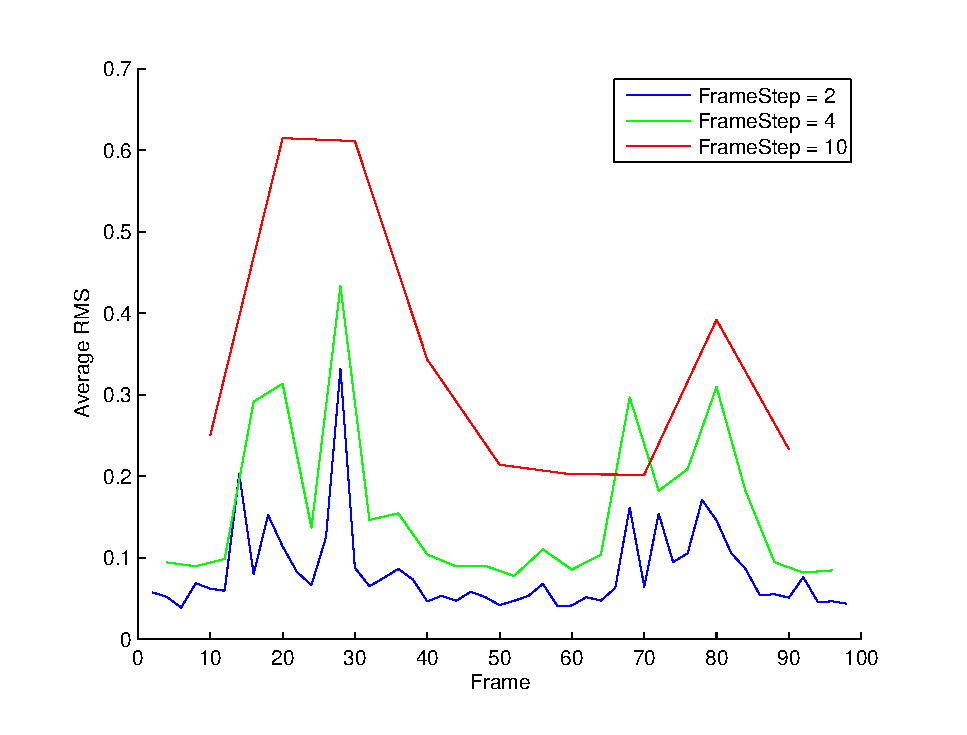
\includegraphics[width=0.98\textwidth]{figures/RMSmergedKD.eps}
    \caption{Average relative RMS error metric for merged kd-tree implementation for frame-step $1,2,4,10$.}
    \label{fig:rmsmergederror}
\end{figure*}

\begin{figure*}[ht!]
  \centering
    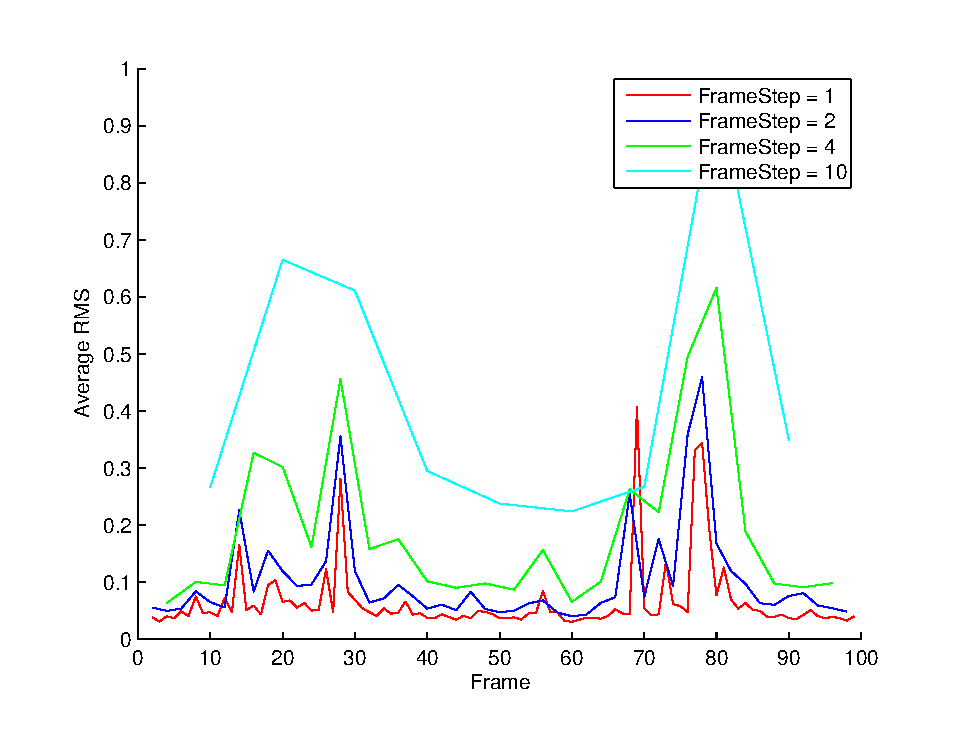
\includegraphics[width=0.98\textwidth]{figures/RMSunmergedKD.eps}
    \caption{Average relative RMS error metric for kd-tree implementation without merging for frame-step $1,2,4,10$.}
    \label{fig:rmsunmergederror}
\end{figure*}

A few variants have been applied~\cite{icpVar} on the ICP algorithm, in which performance improvements resulted from different techniques for, closest point selection, point rejection and error metric variations. For point selection instead of using all available points, a uniform sub-sampling or random sampling among them can lead to faster detection of the closest points. Also, selecting points from more informative regions of the surfaces can lead to better performance since more points are needed if the gradients of the surface are of higher value. As far as matching points are concerned, we can use a few variants apart from searching the whole space of the target surface. A projection of each point in the reference surface to the target one can give us an accurate estimation about where the closest point lies. Also color and angle measurements between surfaces can give us useful information about where to find these points.

\subsection{Dataset}
Our dataset consists of $100$ 3D point clouds that represent surfaces deriving from multiple views of a human body. Figure~\ref{fig:dataset.eps} pictures the point cloud surface.



\subsection{Implementation}
% ADD SOME EQUATIONS HERE
In order to implement our algorithm we followed the work done in ``Implementation of a 3D ICP-based Scan Matches''~\cite{icpImp}. The first and most computationally expensive step of the algorithm is to find for each point of the target cloud the closest point there is in the base one. After doing this we end up having two sets of points with size equal to the target cloud's size. These point clouds need to be centered so we can eliminate any translation the target point cloud might have. Thus, we normalize the base and target cloud's closest point sets subtracting their centers from each of their points. Applying singular value decomposition to the two normalized clouds helps us estimate the rotation of the target cloud with respect to the base. This process continues recomputing the closest points of each cloud and re-transforming the target cloud until the error is minimized.

Given the rotation, we transform the center of the target cloud by multiplying the homogeneous coordinates of it with the estimated rotation matrix subtracting it from the base cloud's center point. The resulting 3D point will serve as the translation of the target cloud with respect to the base one. Applying the estimated translation and rotation transformation onto the target cloud we acquire the new target cloud from which we can now compute the average euclidean distance from the base cloud. This process runs iteratively until the average euclidean distance is minimized.

Another important aspect of the algorithm is the way the merging of the two point clouds is done. There are two methods applied, the first is to merge the two point clouds as one and consider it as the base cloud comparing it with the next frame, and the second one is to store the merged point cloud and proceed considering the target cloud of the first iteration as the base cloud of the second.



\begin{figure*}[bt!]
  \centering
    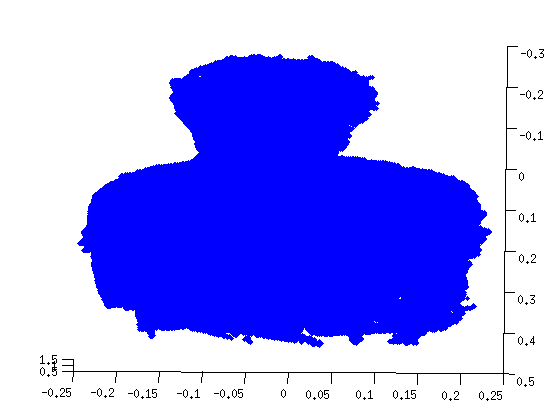
\includegraphics[width=0.24\textwidth]{figures/unBf10.png}\	
    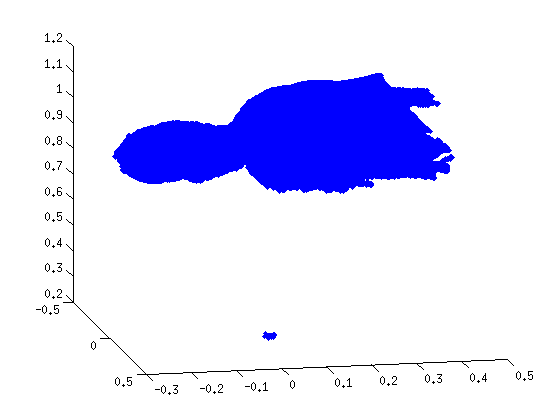
\includegraphics[width=0.24\textwidth]{figures/meUs4.png}\	
    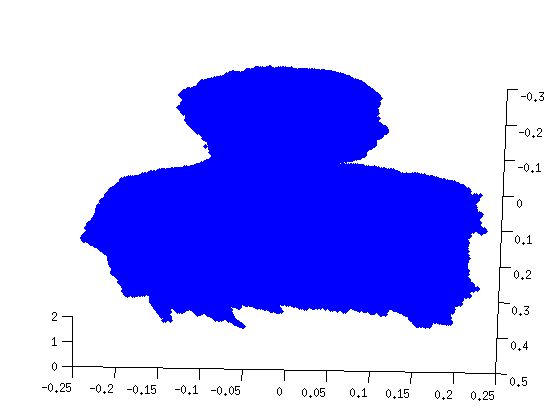
\includegraphics[width=0.24\textwidth]{figures/meKd2.png}\	
    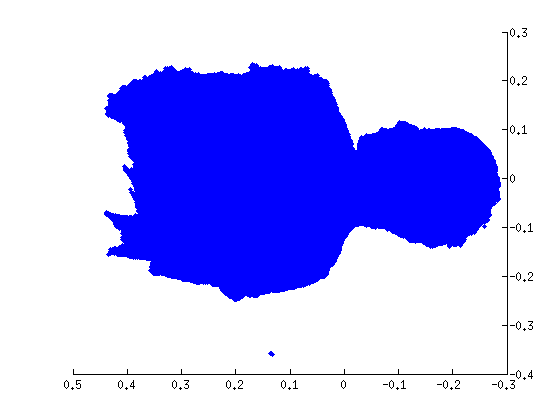
\includegraphics[width=0.24\textwidth]{figures/unKd1.png}
    \caption{Visualization of the merged pointclouds using the ICP algorithm with different closest point selection techniques. From left to right: a) brute force, frame step $10$, no merging b) Uniform sampling, frame step $4$, with merging c) KD-tree, frame step $2$, with merging d) KD-tree, frame step $1$, without merging. }
    \label{fig:mergedICP}
\end{figure*}

\subsection{Results}




\subsection{Discussing the ICP algorithm}
Using the estimated camera poses, merge the point-clouds of all the scenes into one point-cloud and visualize the result. Does the merging produce sufficient result? Discuss why. Now, estimate the camera pose and merge the results using every 2 nd , 4 th , and 10 th frames. Does the camera pose estimation change?




So the estimated camera poses change in comparison with the previous estimates (Sec- tion 2.1)? Does this estimation produce better results?

Even though the ICP algorithm produces sufficient results for surface registration it still has major drawbacks when it comes to its computational cost which makes it really time demanding. The techniques presented earlier in this section improve its complexity without harming the performance. Another issue that arises when it comes to the performance of the algorithm is the fact that the surfaces to be merged need to be close to each other in terms of camera viewpoint, so the merging will converge to a quality solution.

2. How do you think the ICP algorithm can be improved, beside the techniques mentioned in [2], in terms of efficiency and accuracy?


